\documentclass[aspectratio=169,12pt,t]{beamer}

% --- Theme: Metropolis (modern, clean) ---
\usetheme[progressbar=frametitle,numbering=fraction,block=fill]{metropolis}

% --- Fira Sans font (install texlive-fonts-extra if missing) ---
\IfFileExists{FiraSans.sty}{\usepackage[sfdefault]{FiraSans}}{}

% --- Light background with warm accent ---
\definecolor{mDarkTeal}{RGB}{35,55,59}
\definecolor{mLightBrown}{RGB}{235,228,216}
\definecolor{mAccent}{RGB}{140,70,20}

\setbeamercolor{normal text}{fg=mDarkTeal,bg=white}
\setbeamercolor{alerted text}{fg=mAccent}
\setbeamercolor{frametitle}{bg=mDarkTeal,fg=white}
\setbeamercolor{progress bar}{fg=mAccent,bg=mLightBrown}
\setbeamercolor{title separator}{fg=mAccent}
\setbeamercolor{progress bar in head/foot}{fg=mAccent,bg=mLightBrown}
\setbeamercolor{progress bar in section page}{fg=mAccent,bg=mLightBrown}

% --- Packages ---
\usepackage[utf8]{inputenc}
\usepackage{amsmath,amssymb,amsthm}
\usepackage{mathrsfs}
\usepackage{tikz}
\usetikzlibrary{arrows.meta,positioning,calc,decorations.pathreplacing,shapes,patterns}
\usepackage{pgfplots}
\pgfplotsset{compat=1.18}

% --- TikZ diagram styles (shared across the series) ---
\tikzset{
  axisln/.style={-{Stealth[length=2.6mm]}, line width=0.8pt, gray!75},
  curveln/.style={line width=1.6pt, line cap=round, line join=round},
  projln/.style={dash pattern=on 2.6pt off 2pt, line width=0.7pt},
  guide/.style={-{Stealth[length=2.6mm,width=2.2mm]}, line width=1.1pt},
}
% point marker with a white halo: \dotpt{color}{(coord)}
\newcommand{\dotpt}[2]{%
  \fill[white] #2 circle (3.6pt);
  \fill[#1] #2 circle (2.4pt);
}
% open point marker: \opendotpt{color}{(coord)}
\newcommand{\opendotpt}[2]{%
  \fill[white] #2 circle (3.6pt);
  \draw[#1, line width=1pt] #2 circle (2.4pt);
}

% --- Semi-transparent white highlight for text on top of background images ---
\usepackage[most]{tcolorbox}

% Inline highlight: \hl{short text}
\newtcbox{\hl}{%
  nobeforeafter, tcbox raise base,
  colback=white, opacityback=0.6,
  colframe=white, opacityframe=0,
  sharp corners, boxsep=2pt, left=3pt, right=3pt, top=2pt, bottom=2pt%
}

% Block highlight: \begin{hlbox} ... \end{hlbox}  (multi-line, paragraphs, itemize)
% Optional argument accepts any tcolorbox key, e.g. [width=0.6\linewidth]
\newtcolorbox{hlbox}[1][]{%
  enhanced, breakable,
  colback=white, opacityback=0.6,
  colframe=white, opacityframe=0,
  boxsep=3pt, left=6pt, right=6pt, top=4pt, bottom=4pt,
  sharp corners,
  {#1}%
}

% --- Custom colors for content types ---
\definecolor{defcolor}{RGB}{25,85,120}
\definecolor{thmcolor}{RGB}{140,35,35}
\definecolor{proofcolor}{RGB}{35,100,50}
\definecolor{excolor}{RGB}{140,75,10}
\definecolor{remcolor}{RGB}{90,90,90}

% --- Beamer blocks for mathematical content types (semi-transparent) ---
\tcbset{hlblockbase/.style={
  enhanced, breakable,
  coltitle=white, fonttitle=\bfseries,
  opacitybacktitle=0.8, opacityback=0.6,
  opacityframe=0,
  sharp corners,
  boxsep=1pt, left=5pt, right=5pt, top=2pt, bottom=2pt,
  toptitle=1pt, bottomtitle=1pt
}}

\newtcolorbox{defblock}[1]{hlblockbase, title={#1},
  colbacktitle=defcolor, colback=defcolor!15, colframe=defcolor}
\newtcolorbox{thmblock}[1]{hlblockbase, title={#1},
  colbacktitle=thmcolor, colback=thmcolor!15, colframe=thmcolor}
\newtcolorbox{proofblock}[1]{hlblockbase, title={#1},
  colbacktitle=proofcolor, colback=proofcolor!15, colframe=proofcolor}
\newtcolorbox{exblock}[1]{hlblockbase, title={#1},
  colbacktitle=excolor, colback=excolor!15, colframe=excolor}
\newtcolorbox{remblock}[1]{hlblockbase, title={#1},
  colbacktitle=remcolor, colback=remcolor!15, colframe=remcolor}

% --- Metadata ---
\title{Chapter 5: Differentiation}
\subtitle{Section: Derivatives of Higher Order}
\author{Based on Walter Rudin's \emph{Principles of Mathematical Analysis}}
\date{}

\begin{document}

{
\usebackgroundtemplate{%
  
\includegraphics[width=\paperwidth,height=\paperheight,keepaspectratio=false]{chapter_05_bg_00.png}%
}
\begin{frame}[plain]
  \titlepage

  \note{
    Welcome to Chapter 5, Section 5: Derivatives of Higher Order. In the
    previous episodes we defined the derivative of a real function, proved
    the mean value theorems, saw that derivatives have the intermediate
    value property, and put everything to work in Lopital's rule. In this
    short episode we take a simple but far reaching step: the derivative of
    a function is itself a function, so nothing stops us from
    differentiating it again, and again, and again. This gives the second
    derivative, the third derivative, and in general the derivative of
    order "n". Getting the definition and its fine print exactly right is
    the goal of this section, and it is the doorway to Taylor's theorem,
    which is coming in the next episode. Let's dive in.
  }
\end{frame}
}

{
\usebackgroundtemplate{%
  
\includegraphics[width=\paperwidth,height=\paperheight,keepaspectratio=false]{chapter_05_bg_01.png}%
}
\begin{frame}[c]{Outline}
  \begin{center}
    \tableofcontents
  \end{center}

  \note{
    Here is the plan for this episode. We start with motivation: why would
    we want to differentiate more than once, and what do repeated
    derivatives measure. We then state Definition 5.14, which introduces
    the second derivative and the whole tower of higher order derivatives,
    and we fix the notation. Two short examples show the two possible
    behaviors: a polynomial, where derivatives of every order exist, and a
    function whose tower of derivatives stops after one step. After that we
    look carefully at the fine print of the definition: what exactly must
    be true near a point for the derivative of order "n" to exist there.
    Finally we summarize and preview Taylor's theorem.
  }
\end{frame}

\section{Motivation}

% --- Build 1/3 ---
\begin{frame}{Why Differentiate Again?}
  \begin{hlbox}
  \begin{itemize}
    \item The derivative $f'$ answers: \alert{how fast} does $f$ change?
  \end{itemize}
  \end{hlbox}

  \note{
    Let's set the stage. The derivative "f" prime, which we constructed in
    Section 1 of this chapter, answers a single question: at each point,
    how fast is the function "f" changing? Geometrically it is the slope of
    the tangent line to the graph. But this answer immediately suggests a
    follow up question.
  }
\end{frame}

% --- Build 2/3 ---
\begin{frame}{Why Differentiate Again?}
  \begin{hlbox}
  \begin{itemize}
    \item The derivative $f'$ answers: \alert{how fast} does $f$ change?
    \item But $f'$ is itself a \alert{function} on the interval ---
      so we can ask the same question about $f'$:
      \[
        f'' = (f')' \quad \text{measures how the \emph{rate} changes}
      \]
  \end{itemize}
  \end{hlbox}

  \note{
    Here is the key observation. The derivative "f" prime is not just a
    number at one point; it is a function in its own right, defined on the
    interval wherever it exists. And whenever we have a function, we can
    ask our favorite question about it: how fast does it change? Applying
    the derivative to "f" prime gives a new function, written "f" double
    prime, which measures how the rate of change is itself changing. On a
    graph, this is the bending of the curve: whether the slope is
    increasing or decreasing as we move along.
  }
\end{frame}

% --- Build 3/3 ---
\begin{frame}{Why Differentiate Again?}
  \begin{hlbox}
  \begin{itemize}
    \item The derivative $f'$ answers: \alert{how fast} does $f$ change?
    \item But $f'$ is itself a \alert{function} on the interval ---
      so we can ask the same question about $f'$:
      \[
        f'' = (f')' \quad \text{measures how the \emph{rate} changes}
      \]
    \item Iterating gives $f''$, $f^{(3)}$, \dots, $f^{(n)}$ ---
      the raw material of \alert{Taylor's theorem} (next episode)
  \end{itemize}
  \end{hlbox}

  \note{
    And of course there is no reason to stop at two. Differentiating again
    and again, as long as the derivatives keep existing, produces the third
    derivative, the fourth derivative, and in general the derivative of
    order "n". These higher order derivatives are far more than a
    curiosity: they are exactly the raw material of Taylor's theorem, which
    we will prove in the next episode, and which approximates a function by
    a polynomial built from the values of its higher derivatives at a
    single point. First, let's look at a familiar physical example.
  }
\end{frame}

\begin{frame}[c]{A Familiar Instance: Motion}
  \begin{exblock}{Position, velocity, acceleration}
    If $s(t)$ is the position of a particle at time $t$, then
    $s'$ is its \alert{velocity} and $s''$ is its \alert{acceleration}.
  \end{exblock}

  \vspace{0.8em}
  \begin{center}
  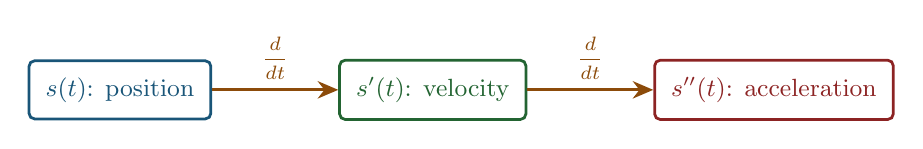
\begin{tikzpicture}[node distance=1.6cm]
    \node[draw=defcolor, line width=1pt, rounded corners=2pt,
      inner sep=6pt, font=\small, text=defcolor] (s) {$s(t)$: position};
    \node[draw=proofcolor, line width=1pt, rounded corners=2pt,
      inner sep=6pt, font=\small, text=proofcolor, right=of s]
      (v) {$s'(t)$: velocity};
    \node[draw=thmcolor, line width=1pt, rounded corners=2pt,
      inner sep=6pt, font=\small, text=thmcolor, right=of v]
      (a) {$s''(t)$: acceleration};
    \draw[guide, excolor] (s) -- (v)
      node[midway, above, font=\scriptsize, text=excolor]
      {$\dfrac{d}{dt}$};
    \draw[guide, excolor] (v) -- (a)
      node[midway, above, font=\scriptsize, text=excolor]
      {$\dfrac{d}{dt}$};
  \end{tikzpicture}
  \end{center}

  \note{
    Higher derivatives are already familiar from physics. Suppose "s" of
    "t" gives the position of a particle at time "t". Each amber arrow in
    the diagram is labeled "d" by "d" "t", meaning: differentiate with
    respect to time. Following the first arrow produces the
    velocity: how fast the position changes. Following the second arrow
    produces the acceleration: how fast the velocity changes. The blue box is the position, the green box the
    velocity, and the red box the acceleration. Newton's second law says
    that force is mass times acceleration, so the second derivative sits at
    the very heart of mechanics. Even the third derivative has a name in
    engineering: it is called the jerk, the rate of change of acceleration.
    With this picture in mind, let's give the formal definition.
  }
\end{frame}
}

{
\usebackgroundtemplate{%
  
\includegraphics[width=\paperwidth,height=\paperheight,keepaspectratio=false]{chapter_05_bg_02.png}%
}
\section{The Definition}

% --- Build 1/2 ---
\begin{frame}{Definition 5.14: Higher Order Derivatives}
  \begin{defblock}{Definition 5.14 (first part)}
    If $f$ has a derivative $f'$ on an interval, and if $f'$ is itself
    differentiable, we denote the derivative of $f'$ by $f''$ and call
    $f''$ the \alert{second derivative} of $f$.
  \end{defblock}

  \note{
    Here is Definition 5.14, in two installments. Suppose first that "f"
    has a derivative "f" prime, not merely at one point but on a whole
    interval. If this new function "f" prime is itself differentiable, its
    derivative is written "f" double prime, and we call it the second
    derivative of "f". Notice the two separate requirements packed into
    this sentence: "f" prime must exist on an interval, so that it makes
    sense to differentiate it, and then "f" prime must actually be
    differentiable. We will return to this fine print shortly. Now let's
    continue the process.
  }
\end{frame}

% --- Build 2/2 ---
\begin{frame}{Definition 5.14: Higher Order Derivatives}
  \begin{defblock}{Definition 5.14 (first part)}
    If $f$ has a derivative $f'$ on an interval, and if $f'$ is itself
    differentiable, we denote the derivative of $f'$ by $f''$ and call
    $f''$ the \alert{second derivative} of $f$.
  \end{defblock}

  \begin{defblock}{Definition 5.14 (continued)}
    Continuing in this manner, we obtain functions
    \[
      f,\ f',\ f'',\ f^{(3)},\ \dots,\ f^{(n)},
    \]
    each of which is the derivative of the preceding one. $f^{(n)}$ is
    called the \alert{$n$th derivative}, or the
    \alert{derivative of order $n$}, of $f$.
  \end{defblock}

  \note{
    Continuing in the same manner, we obtain a whole chain of functions:
    "f", then "f" prime, then "f" double prime, then the third derivative,
    and so on up to the derivative of order "n". Each function in the
    chain is, by definition, the derivative of the one before it. From the
    third derivative onward we abandon the primes, which would become
    unreadable, and instead write the order as a parenthesized superscript.
    The function at the top of the chain is called the derivative of
    order "n" of "f". Let's picture this chain as a tower.
  }
\end{frame}

\begin{frame}[c]{The Tower of Derivatives}
  \begin{center}
  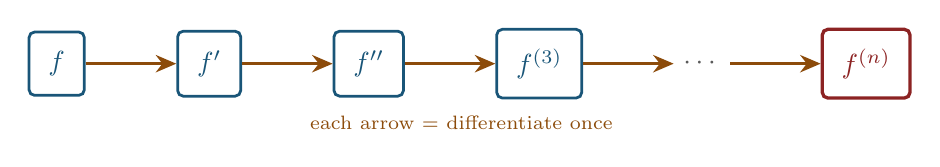
\begin{tikzpicture}[node distance=1.15cm]
    \node[draw=defcolor, line width=1pt, rounded corners=2pt,
      inner sep=7pt, font=\normalsize, text=defcolor] (f0) {$f$};
    \node[draw=defcolor, line width=1pt, rounded corners=2pt,
      inner sep=7pt, font=\normalsize, text=defcolor, right=of f0]
      (f1) {$f'$};
    \node[draw=defcolor, line width=1pt, rounded corners=2pt,
      inner sep=7pt, font=\normalsize, text=defcolor, right=of f1]
      (f2) {$f''$};
    \node[draw=defcolor, line width=1pt, rounded corners=2pt,
      inner sep=7pt, font=\normalsize, text=defcolor, right=of f2]
      (f3) {$f^{(3)}$};
    \node[font=\normalsize, text=remcolor, right=of f3] (fd) {$\cdots$};
    \node[draw=thmcolor, line width=1.2pt, rounded corners=2pt,
      inner sep=7pt, font=\normalsize, text=thmcolor, right=of fd]
      (fn) {$f^{(n)}$};
    \draw[guide, excolor] (f0) -- (f1);
    \draw[guide, excolor] (f1) -- (f2);
    \draw[guide, excolor] (f2) -- (f3);
    \draw[guide, excolor] (f3) -- (fd);
    \draw[guide, excolor] (fd) -- (fn);
    \node[font=\scriptsize, text=excolor, yshift=-0.75cm]
      at ($(f0)!0.5!(fn)$) {each arrow $=$ differentiate once};
  \end{tikzpicture}

  \vspace{1.0em}
  \begin{minipage}{0.8\linewidth}
    \begin{hlbox}
    \begin{itemize}
      \item Each stage must exist before the next one
      \item The chain may continue forever --- or \alert{stop}
    \end{itemize}
    \end{hlbox}
  \end{minipage}
  \end{center}

  \note{
    The picture on the slide shows the tower of derivatives. We start on
    the left with "f" itself, in blue, and every amber arrow means:
    differentiate once. One arrow takes us to "f" prime, another to "f"
    double prime, then to the third derivative, and after finitely many
    steps we reach the derivative of order "n", highlighted in red on the
    right. Two remarks about this tower. First, it is built strictly floor
    by floor: each stage must exist before the next one can even be
    defined, since each function in the chain is the derivative of the
    preceding one. Second, there is no guarantee the tower goes on forever.
    For some functions it does; for others it stops after finitely many
    steps. Let's see one example of each kind.
  }
\end{frame}

\begin{frame}[c]{Example: A Polynomial Never Stops}
  \begin{exblock}{Example: $f(x) = x^3$}
    \[
      f'(x) = 3x^2, \quad
      f''(x) = 6x, \quad
      f^{(3)}(x) = 6, \quad
      f^{(4)}(x) = 0, \quad
      f^{(n)}(x) = 0 \ \ (n \geq 4)
    \]
    Derivatives of \alert{every} order exist, at every point.
  \end{exblock}

  \vspace{0.5em}
  \begin{remblock}{More generally}
    Every polynomial of degree $d$ has derivatives of all orders;\\
    $f^{(n)} \equiv 0$ for all $n > d$.
  \end{remblock}

  \note{
    First, an example where the tower never stops. Take "f" of "x" equal
    to "x" cubed. Differentiating once gives three "x" squared;
    differentiating again gives six "x"; a third time gives the constant
    six; and a fourth time gives zero. From then on, every further
    derivative is the zero function, and the zero function is perfectly
    differentiable, so the tower continues forever. As the gray remark
    notes, the same happens for any polynomial: derivatives of all orders
    exist everywhere, and beyond the degree of the polynomial they are all
    identically zero. So polynomials are as smooth as a function can
    possibly be. But not every function is so accommodating.
  }
\end{frame}

\begin{frame}[c]{Example: The Tower Can Stop}
  \begin{exblock}{Example: $f(x) = x\lvert x\rvert$}
    $f'(x) = 2\lvert x\rvert$ exists for \alert{every} $x$, but $f'$ has a
    \alert{corner} at $0$.\\
    So $f''(0)$ does \alert{not} exist.
  \end{exblock}

  \begin{center}
  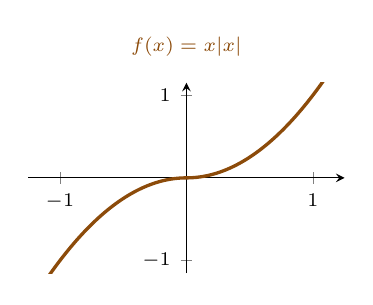
\begin{tikzpicture}
    \begin{axis}[
      width=5.6cm, height=4.0cm,
      axis lines=middle,
      xmin=-1.25, xmax=1.25, ymin=-1.15, ymax=1.15,
      xtick={-1,1}, ytick={-1,1},
      tick label style={font=\scriptsize},
      title style={font=\scriptsize, text=excolor},
      title={$f(x) = x\lvert x\rvert$},
    ]
      \addplot[excolor, line width=1.2pt, domain=-1.1:1.1, samples=120]
        ({x}, {x*abs(x)});
    \end{axis}
  \end{tikzpicture}
  \hspace{0.8cm}
  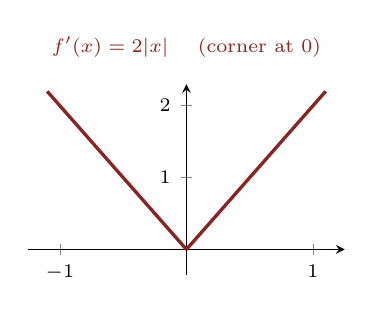
\begin{tikzpicture}
    \begin{axis}[
      width=5.6cm, height=4.0cm,
      axis lines=middle,
      xmin=-1.25, xmax=1.25, ymin=-0.35, ymax=2.3,
      xtick={-1,1}, ytick={1,2},
      tick label style={font=\scriptsize},
      title style={font=\scriptsize, text=thmcolor},
      title={$f'(x) = 2\lvert x\rvert$ \quad (corner at $0$)},
    ]
      \addplot[thmcolor, line width=1.2pt, domain=-1.1:0, samples=2]
        ({x}, {-2*x});
      \addplot[thmcolor, line width=1.2pt, domain=0:1.1, samples=2]
        ({x}, {2*x});
    \end{axis}
  \end{tikzpicture}
  \end{center}

  \note{
    Now an example where the tower stops after one step. Define "f" of "x"
    to be "x" times the absolute value of "x"; that is, "x" squared for
    positive "x" and minus "x" squared for negative "x". The left picture
    shows its graph in amber: a smooth looking "S" shaped curve through
    the origin. This function is differentiable everywhere, and its
    derivative is two times the absolute value of "x". But look at the
    right picture, in red: the graph of "f" prime is a "V" with a sharp
    corner at the
    origin. A corner is exactly where differentiability fails, so the
    second derivative of "f" does not exist at zero, although it exists at
    every other point. The tower for this function has just two complete
    floors. This example shows that the existence of higher derivatives is
    a real restriction, which brings us to the fine print of Definition
    5.14.
  }
\end{frame}
}

{
\usebackgroundtemplate{%
  
\includegraphics[width=\paperwidth,height=\paperheight,keepaspectratio=false]{chapter_05_bg_03.png}%
}
\section{When Does the $n$th Derivative Exist?}

% --- Build 1/2 ---
\begin{frame}{The Fine Print of Definition 5.14}
  \begin{remblock}{For $f^{(n)}(x)$ to exist at a point $x$ \dots}
    \begin{itemize}
      \item $f^{(n-1)}(t)$ must exist for all $t$ in a
        \alert{neighborhood} of $x$ \\
        (one-sided if $x$ is an endpoint of the interval)
    \end{itemize}
  \end{remblock}

  \note{
    Here is the fine print, straight from the book. Suppose we want the
    derivative of order "n" to exist at a particular point "x". By
    definition, it is the derivative, taken at "x", of the previous
    function in the tower, the derivative of order "n" minus one. But a
    derivative at "x" is a limit of difference quotients, and to form
    those quotients we need the previous function to be defined at all
    points "t" near "x", not just at "x" itself. So the derivative of
    order "n" minus one must exist in a whole neighborhood of "x". If "x"
    is an endpoint of the interval on which "f" is defined, a one sided
    neighborhood is enough. And there is a second requirement.
  }
\end{frame}

% --- Build 2/2 ---
\begin{frame}{The Fine Print of Definition 5.14}
  \begin{remblock}{For $f^{(n)}(x)$ to exist at a point $x$ \dots}
    \begin{itemize}
      \item $f^{(n-1)}(t)$ must exist for all $t$ in a
        \alert{neighborhood} of $x$ \\
        (one-sided if $x$ is an endpoint of the interval)
      \item $f^{(n-1)}$ must be \alert{differentiable at $x$}:
        \[
          f^{(n)}(x) = \lim_{t \to x}
            \frac{f^{(n-1)}(t) - f^{(n-1)}(x)}{t - x}
        \]
    \end{itemize}
  \end{remblock}

  \note{
    The second requirement is the obvious one: once the derivative of
    order "n" minus one exists near "x", it must actually be
    differentiable at "x". The displayed formula spells this out: the
    derivative of order "n" at "x" is the limit, as "t" tends to "x", of
    the difference quotient built from the derivative of order "n" minus
    one. This is nothing more than Definition 5.1, the definition of the
    derivative from the start of this chapter, applied to the function one
    floor down. So both ingredients matter: existence of the previous derivative
    on a neighborhood, and differentiability of that previous derivative
    at the point itself. But notice that the first requirement quietly
    reaches even further down the tower.
  }
\end{frame}

\begin{frame}{The Requirement Cascades Down the Tower}
  \begin{remblock}{Cascade}
    Since $f^{(n-1)}$ must exist in a neighborhood of $x$,
    $f^{(n-2)}$ must be \alert{differentiable in that whole neighborhood}
    --- and so on, down the tower.
  \end{remblock}

  \begin{center}
  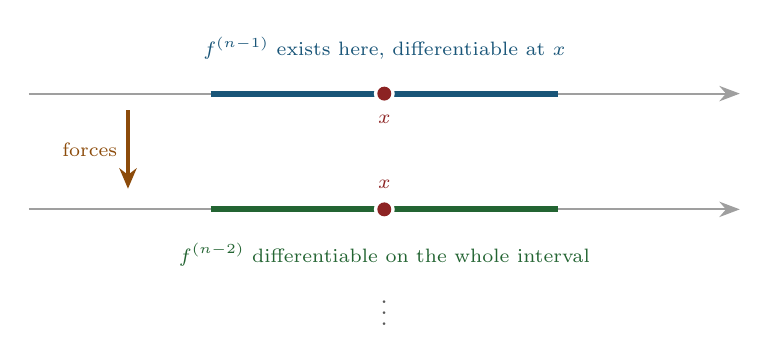
\begin{tikzpicture}[scale=1.05]
    % level n-1
    \node[defcolor, font=\scriptsize] at (4.5,2.55)
      {$f^{(n-1)}$ exists here, differentiable at $x$};
    \draw[axisln] (0.2,2.0) -- (8.8,2.0);
    \draw[defcolor, line width=2.2pt] (2.4,2.0) -- (6.6,2.0);
    \dotpt{thmcolor}{(4.5,2.0)}
    \node[thmcolor, below, font=\scriptsize] at (4.5,1.86) {$x$};
    % level n-2
    \draw[axisln] (0.2,0.6) -- (8.8,0.6);
    \draw[proofcolor, line width=2.2pt] (2.4,0.6) -- (6.6,0.6);
    \dotpt{thmcolor}{(4.5,0.6)}
    \node[thmcolor, above, font=\scriptsize] at (4.5,0.74) {$x$};
    \node[proofcolor, font=\scriptsize] at (4.5,0.05)
      {$f^{(n-2)}$ differentiable on the \alert{whole} interval};
    % cascade arrow
    \draw[guide, excolor] (1.4,1.8) -- (1.4,0.85)
      node[midway, left, font=\scriptsize, text=excolor] {forces};
    \node[remcolor, font=\small] at (4.5,-0.55) {$\vdots$};
  \end{tikzpicture}
  \end{center}

  \note{
    Watch how the requirement propagates. The top number line shows the
    neighborhood of "x", drawn in blue, where the derivative of order "n"
    minus one must exist, with the point "x" marked in red. But at each
    point of that blue interval, the derivative of order "n" minus one is
    itself defined as a derivative. So the function one floor below, of
    order "n" minus two, must be differentiable at every point of that
    interval; that is the green line on the bottom, with the same point
    "x" marked in red, and the amber arrow labeled forces records this
    implication. The same reasoning repeats
    all the way down the tower, as the dots suggest: each lower derivative
    must be differentiable, hence also continuous, on the whole
    neighborhood. So a single number, the derivative of order "n" at one
    point, silently presupposes good behavior of the entire tower on a
    neighborhood of that point. With the definition fully understood,
    let's summarize.
  }
\end{frame}
}

{
\usebackgroundtemplate{%
  
\includegraphics[width=\paperwidth,height=\paperheight,keepaspectratio=false]{chapter_05_bg_04.png}%
}
\section{Summary}

% --- Build 1/3 ---
\begin{frame}{Summary}
  \begin{hlbox}
  \textbf{Key takeaways from this section:}
  \begin{itemize}
    \item \textbf{Definition 5.14:} differentiate repeatedly to get the
      tower $f, f', f'', f^{(3)}, \dots, f^{(n)}$; each function is the
      derivative of the preceding one
  \end{itemize}
  \end{hlbox}

  \note{
    Let's review. This section made one definition, Definition 5.14. The
    derivative of a function is itself a function, so we may differentiate
    repeatedly, obtaining the tower: "f", "f" prime, "f" double prime, the
    third derivative, and so on, up to the derivative of order "n". Each
    function in the tower is by definition the derivative of the one
    before it, and from order three onward we write the order as a
    parenthesized superscript rather than piling up primes. Next, let's
    recall the fine print that comes with this definition.
  }
\end{frame}

% --- Build 2/3 ---
\begin{frame}{Summary}
  \begin{hlbox}
  \textbf{Key takeaways from this section:}
  \begin{itemize}
    \item \textbf{Definition 5.14:} differentiate repeatedly to get the
      tower $f, f', f'', f^{(3)}, \dots, f^{(n)}$; each function is the
      derivative of the preceding one
    \item \textbf{Existence is local and cascading:} $f^{(n)}(x)$ requires
      $f^{(n-1)}$ on a \alert{neighborhood} of $x$, hence $f^{(n-2)}$
      differentiable there, and so on
  \end{itemize}
  \end{hlbox}

  \note{
    Second, the fine print. The derivative of order "n" at a point "x" is
    not a purely pointwise notion: it requires the derivative of order "n"
    minus one to exist on a whole neighborhood of "x" and to be
    differentiable at "x". And this requirement cascades down: every lower
    floor of the tower must be differentiable on that neighborhood. Keep
    this in mind whenever a theorem assumes the existence of a higher
    order derivative; it is quietly assuming a lot of regularity below
    it. Finally, let's remember the two examples.
  }
\end{frame}

% --- Build 3/3 ---
\begin{frame}{Summary}
  \begin{hlbox}
  \textbf{Key takeaways from this section:}
  \begin{itemize}
    \item \textbf{Definition 5.14:} differentiate repeatedly to get the
      tower $f, f', f'', f^{(3)}, \dots, f^{(n)}$; each function is the
      derivative of the preceding one
    \item \textbf{Existence is local and cascading:} $f^{(n)}(x)$ requires
      $f^{(n-1)}$ on a \alert{neighborhood} of $x$, hence $f^{(n-2)}$
      differentiable there, and so on
    \item \textbf{The tower may stop:} $x\lvert x\rvert$ has $f'$
      everywhere but no $f''(0)$; polynomials have derivatives of
      \alert{all} orders
  \end{itemize}

  \vspace{0.6em}
  \textbf{Coming up next:} Taylor's Theorem (5.15) --- approximating $f$
  by a polynomial built from $f(x), f'(x), \dots, f^{(n-1)}(x)$.
  \end{hlbox}

  \note{
    Finally, remember the two examples. The function "x" times the
    absolute value of "x" is differentiable everywhere, yet its second
    derivative fails to exist at zero: the tower can stop. Polynomials, at
    the other extreme, have derivatives of every order at every point. In
    the next episode, this machinery pays off immediately: Taylor's
    theorem, Theorem 5.15, approximates a function by a polynomial whose
    coefficients are built from the values of "f" and its higher
    derivatives at a single point, with the mean value theorem controlling
    the error. It is one of the most useful results in all of analysis.
    See you there.
  }
\end{frame}
}

\end{document}
